\section{Results And Discussion}

	\subsection{Discussion Of Results}
	
	The points of discussion for this experiment are the peaks in the measured spectra. 
	\\
	\\
	At this point, it can be instructive to look at the spectra for Cs-137, which we knew about while performing the experiment. A gamma spectroscopy measurement of Cs-137 can be seen in the figure below.
	\begin{figure}[h]
		\caption{Cs-137 Spectra}
		\centering
		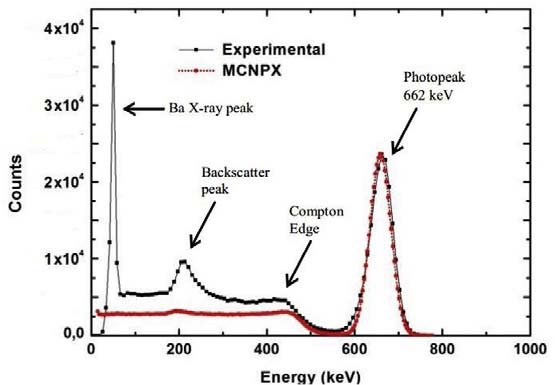
\includegraphics[width=\textwidth]{images/cs137_spectra.png}
	\end{figure}
	\\
	Looking at the three peaks present in the spectra in Figure \ref{fig:CalibrationData}, since we already know the emission spectra of Cs-137, we can easily identify the rightmost and leftmost peaks as the X-ray photopeak, caused by the excitation of lead atoms and the gamma photopeak. Since we know the values for these peaks, we can select the peaks and assign the appropriate value to them for healthier measurements. The smaller peak is the backcatter peak, most probably caused by Compton effect from the shielding inside the detector.
	\\
	\\
	The three peaks discussed in the previous paragraph are present in the experiment data as well as it can be seen in Figure \ref{fig:SmoothedData}, however they are clearly not as sharp as they were in the calibration spectra in Figure \ref{fig:CalibrationData} since radiation coming from other sources have populated the spectra as well. The calibration data was measured when the source was completely adjoining the detector, mitigating all other sources of radiation. However there are many other factors effecting the result and they can be listed as follows:
		\begin{itemize}
			\item The shielding between the radiation source and the detector is not perfect since we have used a lead block to block the direct path. We can clearly see the result of direct radiation in the rightmost small peak in Figure \ref{fig:SmoothedData}.
			\item The second peak from the left is caused by the excitation of the lead block that was encasing the radiation source and this was present in the calibration spectra as well.
			\item The main peaks that we are interested in are not as sharp as the calibration data peaks because the detector most likely measured radiation scattering from the lead blocks all over the experimental setup. This is not much of a problem as well since we can identify the reason and just ignore it, focusing on the two relevant peaks that indicate Compton Effect.
		\end{itemize}
	Smoothing was applied to the data to make it easier to analyze but the results were clear enough in the raw data as well. Compare the figures \ref{fig:RawData} and \ref{fig:SmoothedData} to see the difference that smoothing makes.
	
	\subsection{Discussion Of Errors}
		Although some error was present in the measurement, the results were clear enough to draw concrete conclusions. Especially after the smoothing done by the software of the MCA, errors were less prominent.
	
		\subsubsection{Main Sources Of Errors}
			The main sources of error in this experiment are:
			\\
			\\
				\textbf{Angle Arrangement}: 
					The instrument used for angle arrangement was old and worn down which made it harder for us to see the exact values and align the setup. Also since the instrument was ruler-like, there are vision based errors as well as we used our eyes and hands for alignment. These factors played role in the error of the scattering angle value.
					\\
					\\
				\textbf{Shielding}: 
					Shielding is necessary for safety reasons, however, the excessive shielding of the surroundings and the radiation source itself caused an extra peak in the measured spectra. The radiation that scattered from the lead blocks that are used for shielding effected the result a lot, however since we are aware of this unwanted consequence, we are able to just ignore that peak during the analysis of the main experiment. It was also informative to see the clear consequence of shielding in the resulting spectra which allowed us to brainstorm on it. 
		\subsubsection{Error Mitigation}
			The errors caused by shielding is not very important here since it has little to no effect on the actual peaks that we want to analyze and safety of people in the laboratory is definitely more important than "cleaner data" since the radiation used in this experiment is very dangerous. 
			\\
			\\
			The errors caused by the angle arrangement can be mitigated by replacing the current instrument with a better one, or at least a new one. I think the error in the scattering angle doesn't affect our result very much.